
        \documentclass[12p]{article}
        \usepackage[margin=1in, left=1.5in, includefoot]{geometry}
        \usepackage{longtable, tabu}
        \usepackage[table, dvipsnames]{xcolor}
        \usepackage{array,booktabs}
        \usepackage{color}
        \usepackage{indentfirst}
        \usepackage{graphicx}
        \usepackage{float}
        \usepackage[utf8]{inputenc}
        \usepackage{listings}
        \usepackage{url}
        \usepackage{multirow}
        \usepackage{seqsplit}
        
        \definecolor{ferrarired}{rgb}{1.0, 0.11, 0.0}
        \definecolor{orange(colorwheel)}{rgb}{1.0, 0.5, 0.0}
        \definecolor{deepskyblue}{rgb}{0.0, 0.75, 1.0}
        \definecolor{grannysmithapple}{rgb}{0.66, 0.89, 0.63}
        \definecolor{gray(x11gray)}{rgb}{0.75, 0.75, 0.75}
        \definecolor{amber}{rgb}{1.0, 0.75, 0.0}
        
        \newcommand{\icon}[1]{\includegraphics[height=12pt]{#1}}
        \newcommand{\hash}[1]{{\ttfamily\seqsplit{#1}}}

        \setlength{\arrayrulewidth}{0.3mm}
\setlength{\tabcolsep}{18pt}
\renewcommand{\arraystretch}{1.5}
\setlength{\parindent}{1em}
\begin{document}
\begin{titlepage}
\begin{center}
\line(1,0){320}\\
[0.25in]
\huge{\bfseries Android Analysis Report}
\line(1,0){320}\\
[0.5in]
\begin{figure}[H]
	\centering
	
\includegraphics[scale=0.5]{/home/miki/Documents/GITHUB/AndroidPermissions/python/vulns/report_icons/logo.png}
\end{figure}
\textsl{\LARGE Demo app}\\
\textsf{\LARGE ro.ing.mobile.banking.android.activity}\\
[2.5in]
\end{center}
\begin{flushright}
\textbf{\large Date 2018-06-14}
\end{flushright}
\end{titlepage}
\tableofcontents
\thispagestyle{empty}
\cleardoublepage
\setcounter{page}{1}
\section{PERMISSIONS}
	\begin{longtable}{p{3cm} p{10cm} }
	\rowcolor{grannysmithapple!70} Type & List \\
Normal &  ACCESS\_NETWORK\_STATE \\ 
 &  INSTALL\_SHORTCUT \\ 
 &  INTERNET \\ 
 &  INSTALL\_SHORTCUT \\ 
 &  WAKE\_LOCK \\ 
\hline
Dangerous &  CAMERA \\ 
 &  READ\_CONTACTS \\ 
 &  ACCESS\_COARSE\_LOCATION \\ 
 &  ACCESS\_FINE\_LOCATION \\ 
 &  READ\_PHONE\_STATE \\ 
\hline
Overprivileged &  USE\_FINGERPRINT \\ 
 &  READ\_EXTERNAL\_STORAGE \\ 
 &  C \\ 
 &  VIBRATE \\ 
 &  WRITE\_USE\_APP\_FEATURE\_SURVEY \\ 
 &  GET\_ACCOUNTS \\ 
 &  RECEIVE \\ 
 &  CALL\_PHONE \\ 
 &  READ\_GSERVICES \\ 
\hline
Underprivileged &  "android.permission.INTERNET" \\ 
 &  "android.permission.ACCESS\_NETWORK\_STATE" \\ 
 &  INSTALL\_SHORTCUT \\ 
 &  "android.permission.WAKE\_LOCK" \\ 
\hline
Automatically granted dangerous permissions &  WRITE\_CONTACTS \\ 
 &  ANSWER\_PHONE\_CALLSREAD\_PHONE\_NUMBERS \\ 
 &  READ\_CALL\_LOG \\ 
 &  WRITE\_CALL\_LOG \\ 
 &  ADD\_VOICEMAIL \\ 
 &  USE\_SIP \\ 
 &  PROCESS\_OUTGOING\_CALLS \\ 
 &  WRITE\_EXTERNAL\_STORAGE \\ 
\hline
	\end{longtable}
\section{FINDINGS SUMMARY}\label{sec:summary}
\begin{figure}[H]
\centering
	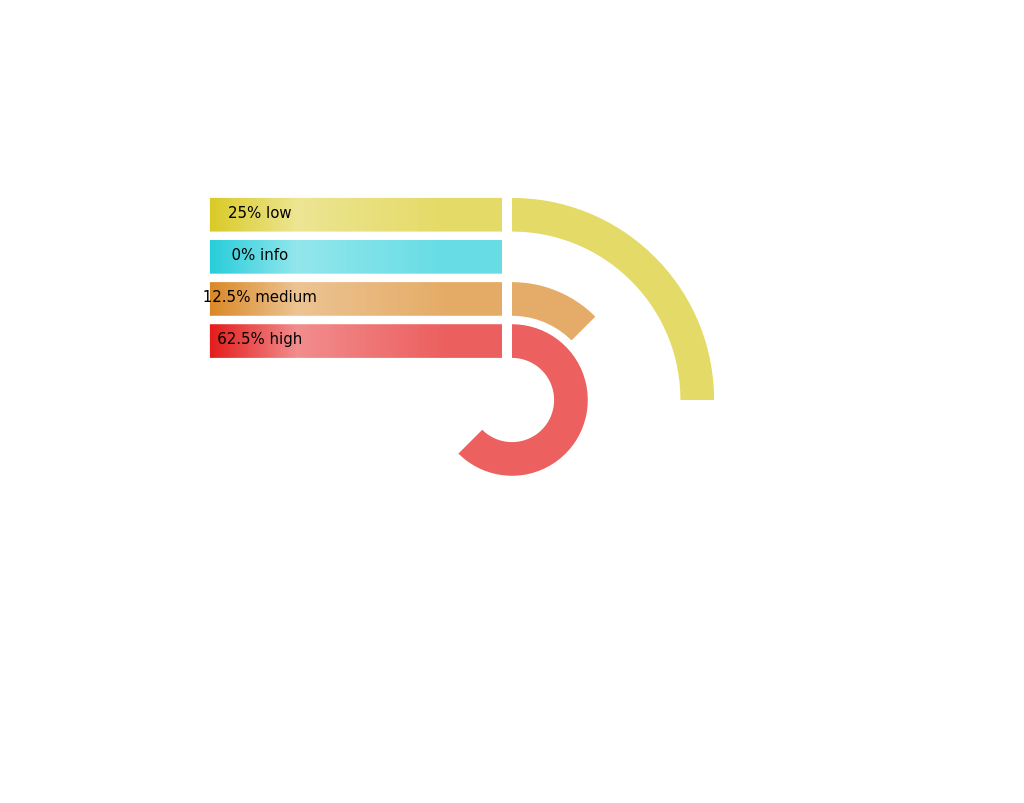
\includegraphics[scale=0.5]{/home/miki/Documents/GITHUB/AndroidPermissions/apks/playstore_apps/ro_ing_mobile_banking_android_activity/report/pie_chart.png}
\end{figure}
	\begin{longtable}{p{0.5cm} p{10cm} p{1.5cm}}
	\rowcolor{grannysmithapple!70} Index & Title & Impact \\
	A1&Access local ressources& \color{ferrarired}\textbf{High} \\
\hline\\	A2&Load cleartext content& \color{ferrarired}\textbf{High} \\
\hline\\	A3&& \color{amber}\textbf{Low} \\
\hline\\	A4&JavascriptInterfaceAnalyser& \color{ferrarired}\textbf{High} \\
\hline\\	A5&Application Data can be Backed up android:allowBackup flag is missing.& \color{orange(colorwheel)}\textbf{Medium} \\
\hline\\	A6&Service \newline (ro. ing. android. notification. InstanceIDListenerService) is not Protected. An intent-filter exists.& \color{ferrarired}\textbf{High} \\
\hline\\	A7&Service \newline (ro. ing. android. notification. FcmListenerService) is not Protected. An intent-filter exists.& \color{ferrarired}\textbf{High} \\
\hline\\	A8&Service \newline (com. google. firebase. messaging. FirebaseMessagingService) is not Protected. [android:exported=true]& \color{ferrarired}\textbf{High} \\
\hline\\	A9&Service \newline (com. google. firebase. iid. FirebaseInstanceIdService) is not Protected. [android:exported=true]& \color{ferrarired}\textbf{High} \\
\hline\\	A10&& \color{amber}\textbf{Low} \\
\hline\\	\end{longtable}
\cleardoublepage
\newpage
\section{DETAILED FINDINGS}
\subsection{A1: Access local ressources}
\subsubsection*{\protect\icon{/home/miki/Documents/GITHUB/AndroidPermissions/python/vulns/report_icons/basic_sheet.png} Description}

\subsubsection*{\protect\icon{/home/miki/Documents/GITHUB/AndroidPermissions/python/vulns/report_icons/basic_magnifier.png} Evidence}
\path{/home/miki/Documents/GITHUB/AndroidPermissions/apks/playstore_apps/ro_ing_mobile_banking_android_activity/app/smali/ro/ing/mobile/banking/android/activity/ClientWebViewActivity.smali}

\subsubsection*{\protect\icon{/home/miki/Documents/GITHUB/AndroidPermissions/python/vulns/report_icons/basic_todo.png} Recommendation}

\subsection{A2: Load cleartext content}
\subsubsection*{\protect\icon{/home/miki/Documents/GITHUB/AndroidPermissions/python/vulns/report_icons/basic_sheet.png} Description}

\subsubsection*{\protect\icon{/home/miki/Documents/GITHUB/AndroidPermissions/python/vulns/report_icons/basic_magnifier.png} Evidence}
\path{/home/miki/Documents/GITHUB/AndroidPermissions/apks/playstore_apps/ro_ing_mobile_banking_android_activity/app/smali/de/neom/neoreadersdk/Viewfinder14View$AdView.smali loadUrl}

\path{/home/miki/Documents/GITHUB/AndroidPermissions/apks/playstore_apps/ro_ing_mobile_banking_android_activity/app/smali/de/neom/neoreadersdk/Viewfinder14View$AdView.smali loadUrl}

\path{/home/miki/Documents/GITHUB/AndroidPermissions/apks/playstore_apps/ro_ing_mobile_banking_android_activity/app/smali/de/neom/neoreadersdk/Viewfinder5View$AdView.smali loadUrl}

\path{/home/miki/Documents/GITHUB/AndroidPermissions/apks/playstore_apps/ro_ing_mobile_banking_android_activity/app/smali/de/neom/neoreadersdk/Viewfinder5View$AdView.smali loadUrl}

\subsubsection*{\protect\icon{/home/miki/Documents/GITHUB/AndroidPermissions/python/vulns/report_icons/basic_todo.png} Recommendation}

\subsection{A3: }
\subsubsection*{\protect\icon{/home/miki/Documents/GITHUB/AndroidPermissions/python/vulns/report_icons/basic_sheet.png} Description}

\subsubsection*{\protect\icon{/home/miki/Documents/GITHUB/AndroidPermissions/python/vulns/report_icons/basic_magnifier.png} Evidence}
\path{/home/miki/Documents/GITHUB/AndroidPermissions/apks/playstore_apps/ro_ing_mobile_banking_android_activity/app/smali/メ.smali
Landroid/util/Log -> e(Ljava/lang/String;Ljava/lang/String;)}

\path{/home/miki/Documents/GITHUB/AndroidPermissions/apks/playstore_apps/ro_ing_mobile_banking_android_activity/app/smali/ー$if.smali
Landroid/util/Log -> w(Ljava/lang/String;Ljava/lang/String;)}

\path{/home/miki/Documents/GITHUB/AndroidPermissions/apks/playstore_apps/ro_ing_mobile_banking_android_activity/app/smali/ᖭ.smali
Landroid/util/Log -> i(Ljava/lang/String;Ljava/lang/String;)}

\path{/home/miki/Documents/GITHUB/AndroidPermissions/apks/playstore_apps/ro_ing_mobile_banking_android_activity/app/smali/ﻐ.smali
Landroid/util/Log -> e(Ljava/lang/String;Ljava/lang/String;)}

\path{/home/miki/Documents/GITHUB/AndroidPermissions/apks/playstore_apps/ro_ing_mobile_banking_android_activity/app/smali/ﻐ.smali
Landroid/util/Log -> e(Ljava/lang/String;Ljava/lang/String;)}

\path{/home/miki/Documents/GITHUB/AndroidPermissions/apks/playstore_apps/ro_ing_mobile_banking_android_activity/app/smali/⁔.smali
Landroid/util/Log -> e(Ljava/lang/String;Ljava/lang/String;Ljava/lang/Throwable;)}

\path{/home/miki/Documents/GITHUB/AndroidPermissions/apks/playstore_apps/ro_ing_mobile_banking_android_activity/app/smali/Ϯ.smali
Landroid/util/Log -> d(Ljava/lang/String;Ljava/lang/String;)}

\path{/home/miki/Documents/GITHUB/AndroidPermissions/apks/playstore_apps/ro_ing_mobile_banking_android_activity/app/smali/ᔊ.smali
Landroid/util/Log -> w(Ljava/lang/String;Ljava/lang/String;)}

\path{/home/miki/Documents/GITHUB/AndroidPermissions/apks/playstore_apps/ro_ing_mobile_banking_android_activity/app/smali/ᴱ.smali
Landroid/util/Log -> wtf(Ljava/lang/String;Ljava/lang/String;Ljava/lang/Throwable;)}

\path{/home/miki/Documents/GITHUB/AndroidPermissions/apks/playstore_apps/ro_ing_mobile_banking_android_activity/app/smali/ᴱ.smali
Landroid/util/Log -> w(Ljava/lang/String;Ljava/lang/String;)}


\textit{snip}
\newline \textsl{For the full list view \path{/home/miki/Documents/GITHUB/AndroidPermissions/apks/playstore_apps/ro_ing_mobile_banking_android_activity/report}}
\subsubsection*{\protect\icon{/home/miki/Documents/GITHUB/AndroidPermissions/python/vulns/report_icons/basic_todo.png} Recommendation}

\subsection{A4: JavascriptInterfaceAnalyser}
\subsubsection*{\protect\icon{/home/miki/Documents/GITHUB/AndroidPermissions/python/vulns/report_icons/basic_sheet.png} Description}

\subsubsection*{\protect\icon{/home/miki/Documents/GITHUB/AndroidPermissions/python/vulns/report_icons/basic_magnifier.png} Evidence}
\path{/home/miki/Documents/GITHUB/AndroidPermissions/apks/playstore_apps/ro_ing_mobile_banking_android_activity/app/smali/ro/ing/mobile/banking/android/activity/ClientWebViewActivity.smali addJavascriptInterface}

\path{/home/miki/Documents/GITHUB/AndroidPermissions/apks/playstore_apps/ro_ing_mobile_banking_android_activity/app/smali/de/neom/neoreadersdk/Viewfinder14View$AdView.smali addJavascriptInterface}

\path{/home/miki/Documents/GITHUB/AndroidPermissions/apks/playstore_apps/ro_ing_mobile_banking_android_activity/app/smali/de/neom/neoreadersdk/Viewfinder5View$AdView.smali addJavascriptInterface}

\subsubsection*{\protect\icon{/home/miki/Documents/GITHUB/AndroidPermissions/python/vulns/report_icons/basic_todo.png} Recommendation}

\subsection{A5: Application Data can be Backed up android:allowBackup flag is missing.}
\subsubsection*{\protect\icon{/home/miki/Documents/GITHUB/AndroidPermissions/python/vulns/report_icons/basic_sheet.png} Description}
By default [android:allowBackup] flag is set to true, allowing anyone to backup your application data via adb. It also allows users who have enabled USB debugging to copy application data off of the device.
\subsubsection*{\protect\icon{/home/miki/Documents/GITHUB/AndroidPermissions/python/vulns/report_icons/basic_todo.png} Recommendation}
android:allowBackup = False
\subsection{A6: Service (ro. ing. android. notification. InstanceIDListenerService) is not Protected. An intent-filter exists.}
\subsubsection*{\protect\icon{/home/miki/Documents/GITHUB/AndroidPermissions/python/vulns/report_icons/basic_sheet.png} Description}
A  Service is found to be shared with other apps on the device therefore leaving it accessible to any other application on the device. The presence of intent-filter indicates that the Service is explicitly exported.
\subsubsection*{\protect\icon{/home/miki/Documents/GITHUB/AndroidPermissions/python/vulns/report_icons/basic_todo.png} Recommendation}
It is recommended to set the protection level to signature, so only applications signed with the same certificate can obtain the permission.
\subsection{A7: Service (ro. ing. android. notification. FcmListenerService) is not Protected. An intent-filter exists.}
\subsubsection*{\protect\icon{/home/miki/Documents/GITHUB/AndroidPermissions/python/vulns/report_icons/basic_sheet.png} Description}
A  Service is found to be shared with other apps on the device therefore leaving it accessible to any other application on the device. The presence of intent-filter indicates that the Service is explicitly exported.
\subsubsection*{\protect\icon{/home/miki/Documents/GITHUB/AndroidPermissions/python/vulns/report_icons/basic_todo.png} Recommendation}
It is recommended to set the protection level to signature, so only applications signed with the same certificate can obtain the permission.
\subsection{A8: Service (com. google. firebase. messaging. FirebaseMessagingService) is not Protected. [android:exported=true]}
\subsubsection*{\protect\icon{/home/miki/Documents/GITHUB/AndroidPermissions/python/vulns/report_icons/basic_sheet.png} Description}
A Service is found to be shared with other apps on the device therefore leaving it accessible to any other application on the device.
\subsubsection*{\protect\icon{/home/miki/Documents/GITHUB/AndroidPermissions/python/vulns/report_icons/basic_todo.png} Recommendation}
It is recommended to set the protection level to signature, so only applications signed with the same certificate can obtain the permission.
\subsection{A9: Service (com. google. firebase. iid. FirebaseInstanceIdService) is not Protected. [android:exported=true]}
\subsubsection*{\protect\icon{/home/miki/Documents/GITHUB/AndroidPermissions/python/vulns/report_icons/basic_sheet.png} Description}
A Service is found to be shared with other apps on the device therefore leaving it accessible to any other application on the device.
\subsubsection*{\protect\icon{/home/miki/Documents/GITHUB/AndroidPermissions/python/vulns/report_icons/basic_todo.png} Recommendation}
It is recommended to set the protection level to signature, so only applications signed with the same certificate can obtain the permission.
\subsection{A10: }
\subsubsection*{\protect\icon{/home/miki/Documents/GITHUB/AndroidPermissions/python/vulns/report_icons/basic_sheet.png} Description}

\subsubsection*{\protect\icon{/home/miki/Documents/GITHUB/AndroidPermissions/python/vulns/report_icons/basic_magnifier.png} Evidence}
\path{/home/miki/Documents/GITHUB/AndroidPermissions/apks/playstore_apps/ro_ing_mobile_banking_android_activity/app/smali/ﻪ.smali forName}

\path{/home/miki/Documents/GITHUB/AndroidPermissions/apks/playstore_apps/ro_ing_mobile_banking_android_activity/app/smali/ᒌ.smali forName}

\path{/home/miki/Documents/GITHUB/AndroidPermissions/apks/playstore_apps/ro_ing_mobile_banking_android_activity/app/smali/ᒶ.smali invoke}

\path{/home/miki/Documents/GITHUB/AndroidPermissions/apks/playstore_apps/ro_ing_mobile_banking_android_activity/app/smali/ه.smali invoke}

\path{/home/miki/Documents/GITHUB/AndroidPermissions/apks/playstore_apps/ro_ing_mobile_banking_android_activity/app/smali/য.smali forName}

\path{/home/miki/Documents/GITHUB/AndroidPermissions/apks/playstore_apps/ro_ing_mobile_banking_android_activity/app/smali/ᔲ.smali invoke}

\path{/home/miki/Documents/GITHUB/AndroidPermissions/apks/playstore_apps/ro_ing_mobile_banking_android_activity/app/smali/ষ.smali invoke}

\path{/home/miki/Documents/GITHUB/AndroidPermissions/apks/playstore_apps/ro_ing_mobile_banking_android_activity/app/smali/ষ.smali invoke}

\path{/home/miki/Documents/GITHUB/AndroidPermissions/apks/playstore_apps/ro_ing_mobile_banking_android_activity/app/smali/ﺜ.smali getComponentType}

\path{/home/miki/Documents/GITHUB/AndroidPermissions/apks/playstore_apps/ro_ing_mobile_banking_android_activity/app/smali/ڹ.smali forName}


\textit{snip}
\newline \textsl{For the full list view \path{/home/miki/Documents/GITHUB/AndroidPermissions/apks/playstore_apps/ro_ing_mobile_banking_android_activity/report}}
\subsubsection*{\protect\icon{/home/miki/Documents/GITHUB/AndroidPermissions/python/vulns/report_icons/basic_todo.png} Recommendation}

\cleardoublepage
\newpage
\section{VISUALIZATIONS}
\subsection{Chord Diagram - Class Relations}
\begin{figure}[H]
	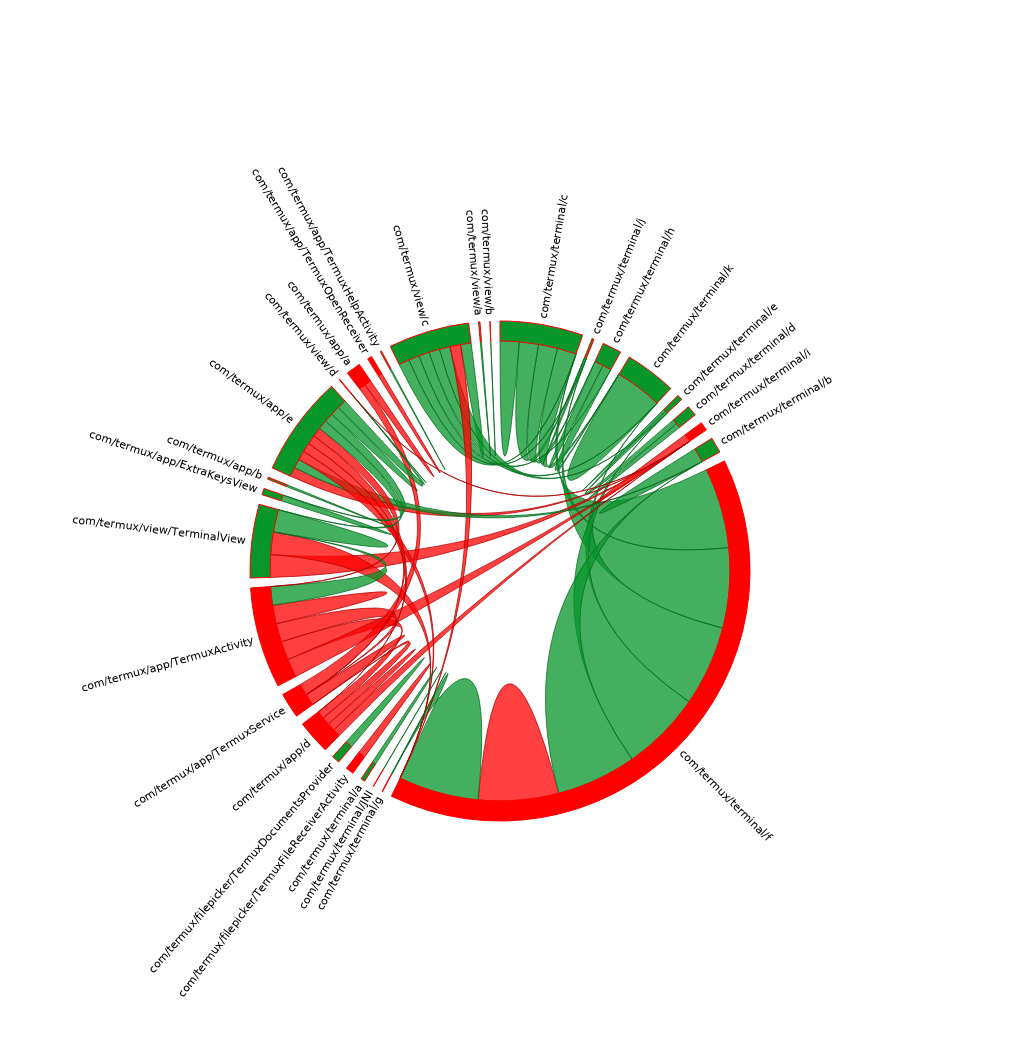
\includegraphics[scale=0.45]{/home/miki/Documents/GITHUB/AndroidPermissions/apks/playstore_apps/ro_ing_mobile_banking_android_activity/report/chord_diagram.png}\end{figure}\subsection{Hot Spot - System Overview}
\begin{figure}[H]
\centering
	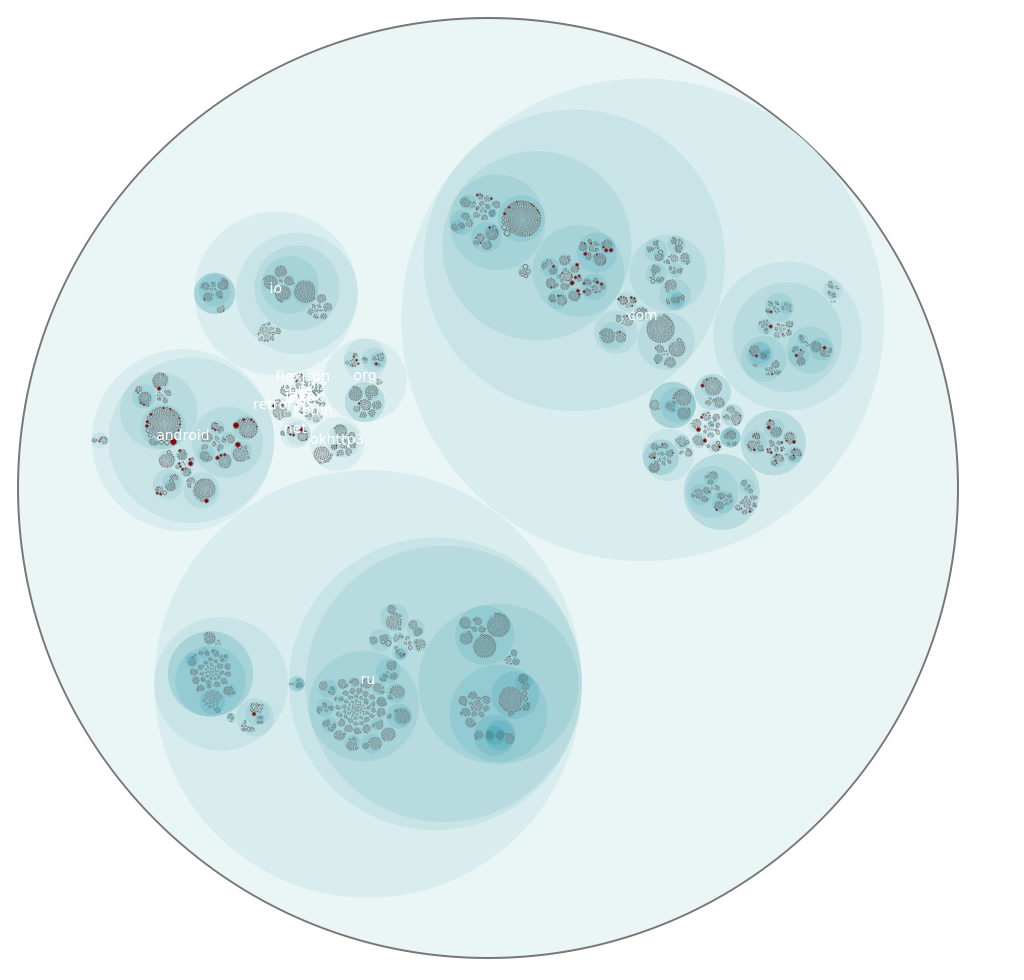
\includegraphics[scale=0.5]{/home/miki/Documents/GITHUB/AndroidPermissions/apks/playstore_apps/ro_ing_mobile_banking_android_activity/report/hotspot.png}\end{figure}\begin{longtable}{p{0.3cm} p{12cm}}
\rowcolor{orange} Index & Class \\
1 & \path{/home/miki/Documents/GITHUB/AndroidPermissions/apks/playstore_apps/ro_ing_mobile_banking_android_activity/app/smali/de/neom/neoreadersdk/Viewfinder5View.smali} \\
2 & \path{/home/miki/Documents/GITHUB/AndroidPermissions/apks/playstore_apps/ro_ing_mobile_banking_android_activity/app/smali/de/neom/neoreadersdk/Viewfinder14View.smali} \\
3 & \path{/home/miki/Documents/GITHUB/AndroidPermissions/apks/playstore_apps/ro_ing_mobile_banking_android_activity/app/smali/ro/ing/mobile/banking/android/activity/ScanActivity$ˊ.smali} \\
4 & \path{/home/miki/Documents/GITHUB/AndroidPermissions/apks/playstore_apps/ro_ing_mobile_banking_android_activity/app/smali/ষ.smali} \\
5 & \path{/home/miki/Documents/GITHUB/AndroidPermissions/apks/playstore_apps/ro_ing_mobile_banking_android_activity/app/smali/android/support/v4/media/MediaBrowserCompat$MediaBrowserImplBase.smali} \\
6 & \path{/home/miki/Documents/GITHUB/AndroidPermissions/apks/playstore_apps/ro_ing_mobile_banking_android_activity/app/smali/android/support/v4/media/session/MediaControllerCompat$TransportControlsBase.smali} \\
7 & \path{/home/miki/Documents/GITHUB/AndroidPermissions/apks/playstore_apps/ro_ing_mobile_banking_android_activity/app/smali/android/support/v4/media/session/MediaControllerCompat$MediaControllerImplBase.smali} \\
8 & \path{/home/miki/Documents/GITHUB/AndroidPermissions/apks/playstore_apps/ro_ing_mobile_banking_android_activity/app/smali/ro/ing/mobile/banking/android/activity/ScanActivity.smali} \\
9 & \path{/home/miki/Documents/GITHUB/AndroidPermissions/apks/playstore_apps/ro_ing_mobile_banking_android_activity/app/smali/de/neom/neoreadersdk/ViewfinderActivity.smali} \\
10 & \path{/home/miki/Documents/GITHUB/AndroidPermissions/apks/playstore_apps/ro_ing_mobile_banking_android_activity/app/smali/ต.smali} \\
	\end{longtable}
\end{document}
